% !TeX program = xelatex
\documentclass[a4paper,10pt]{article}

% ============================================================================
% កញ្ចប់បណ្ណាល័យ (Packages) – តាមលំនាំ NGS Preah Krasang (ls_plan.tex)
% បរិបទ៖ គ្មានស្លាយ LCD និងគ្មានម៉ាស៊ីនគិតលេខ — ប្រើសន្លឹកកិច្ចការសិស្ស (ស-ខ្មៅ) និងក្ដារខៀនជាគោល
% ============================================================================
\usepackage[a4paper, left=0.95cm, right=0.95cm, top=0.85cm, bottom=0.92cm, footskip=0.52cm]{geometry}
\usepackage{amsmath, amssymb}
\usepackage{unicode-math}
\usepackage{fontspec}
\usepackage{array, longtable, multirow, colortbl}
\usepackage[table]{xcolor}
\usepackage{enumitem}
\usepackage{pifont}
\usepackage{fancyhdr}
\usepackage{tikz}
\usetikzlibrary{calc, arrows.meta, angles, quotes, decorations.markings, decorations.pathreplacing, patterns, babel}

\makeatletter
\let\@expl@@@mark@update@singlecol@structures@@\relax
\makeatother

\providecommand{\NGSFindFonts}{%
  \IfFileExists{C:/Windows/Fonts/cambria.ttc}{%
    \def\NGSSysPath{C:/Windows/Fonts/}%
    \def\NGSUserPath{C:/Users/KIT/AppData/Local/Microsoft/Windows/Fonts/}%
  }{%
    \IfFileExists{./fonts/KhmerOSsiemreap.ttf}{\def\NGSSysPath{./fonts/}\def\NGSUserPath{./fonts/}}{%
    \IfFileExists{../fonts/KhmerOSsiemreap.ttf}{\def\NGSSysPath{../fonts/}\def\NGSUserPath{../fonts/}}{%
    \IfFileExists{../../fonts/KhmerOSsiemreap.ttf}{\def\NGSSysPath{../../fonts/}\def\NGSUserPath{../../fonts/}}{%
    \IfFileExists{../../../fonts/KhmerOSsiemreap.ttf}{\def\NGSSysPath{../../../fonts/}\def\NGSUserPath{../../../fonts/}}{%
    \IfFileExists{../../../../fonts/KhmerOSsiemreap.ttf}{\def\NGSSysPath{../../../../fonts/}\def\NGSUserPath{../../../../fonts/}}{%
    \IfFileExists{../../../../../fonts/KhmerOSsiemreap.ttf}{\def\NGSSysPath{../../../../../fonts/}\def\NGSUserPath{../../../../../fonts/}}{%
    \IfFileExists{../../../../../../fonts/KhmerOSsiemreap.ttf}{\def\NGSSysPath{../../../../../../fonts/}\def\NGSUserPath{../../../../../../fonts/}}{%
      \def\NGSSysPath{../../../../../../../fonts/}\def\NGSUserPath{../../../../../../../fonts/}%
    }}}}}}}%
  }%
}
\NGSFindFonts

\setmathfont[Path={\NGSSysPath}, FontIndex=1, Scale=1.02]{cambria.ttc}
\defaultfontfeatures{Ligatures=TeX}

\setmainfont[
  Path={\NGSUserPath}, Extension=.ttf, Script=Khmer,
  BoldFont={KhmerOSsiemreap}, BoldFeatures={FakeBold=1.8},
  ItalicFont={KhmerOSsiemreap}, ItalicFeatures={FakeSlant=0.25},
  BoldItalicFont={KhmerOSsiemreap}, BoldItalicFeatures={FakeBold=1.8, FakeSlant=0.25}
]{KhmerOSsiemreap}

\newfontfamily\muol[Path={\NGSUserPath}, Extension=.ttf, Script=Khmer]{KhmerOSmuollight}
\newfontfamily\TimesEn[Path={\NGSSysPath}, Extension=.ttf, Scale=1.00, BoldFont={timesbd}, ItalicFont={timesi}, BoldItalicFont={timesbi}]{times}
\newfontfamily\NagaBold[Path={\NGSUserPath}, Extension=.ttf]{AKbalthom Naga Bold}
\newfontfamily\CalibriFont[Path={\NGSSysPath}, Extension=.ttf]{calibri}
\newfontfamily\Tacteing[Path={\NGSUserPath}]{TACTENG.TTF}
\newfontfamily\CourierBullet[Path={\NGSSysPath}, Extension=.ttf]{cour}
\newcommand{\wcirc}{{\CourierBullet\fontsize{9.5pt}{11pt}\selectfont o}}

\XeTeXlinebreaklocale "km"
\XeTeXlinebreakskip = 0pt plus 1pt minus 0.1pt

\definecolor{stepgray}{HTML}{D9D9D9}
\definecolor{headgray}{HTML}{F2F2F2}
\definecolor{boxgray}{HTML}{D9D9D9}
\definecolor{darkred}{HTML}{C00000}
\definecolor{red5e}{HTML}{FF0000}

\pagestyle{fancy}
\fancyhf{}
\renewcommand{\headrulewidth}{0pt}
\fancyfoot[R]{\CalibriFont\fontsize{11pt}{13pt}\selectfont\thepage}

\setlength{\parindent}{0pt}
\setlength{\parskip}{0pt}
\setlength{\tabcolsep}{3.8pt}

\newcolumntype{L}[1]{>{\raggedright\arraybackslash}p{#1}}
\newcolumntype{C}[1]{>{\centering\arraybackslash}p{#1}}

\newcommand{\en}[1]{{\TimesEn #1}}
\newcommand{\enbf}[1]{{\TimesEn\textbf{#1}}}
\newcommand{\unit}[1]{\,\text{\en{#1}}}
\newcommand{\fiveE}[1]{{\NagaBold\fontsize{9.5pt}{13pt}\selectfont\textcolor{red5e}{#1}}}
\newcommand{\timenote}[1]{\textcolor{darkred}{\textit{#1}}}
\newcommand{\graybox}[1]{\colorbox{boxgray}{\strut\hspace{2pt}#1\hspace{2pt}}}
\newcommand{\cnum}[1]{{\fontsize{10.5pt}{12pt}\selectfont\ding{\numexpr181+#1\relax}}\hspace{0.15em}}
\newcommand{\cfig}[1]{\par\vspace{3pt}{\centering #1\par}\vspace{3pt}}
\newcommand{\stepheader}[1]{\multicolumn{3}{|c|}{\cellcolor{stepgray}\muol #1} \\* \noalign{\hrule height 0.4pt}}
\newcommand{\khmflourish}{{\Tacteing\fontsize{36pt}{14pt}\selectfont\raisebox{-5pt}{3}}}

% ============================================================================
% ម៉ាក្រូគូសរូប TikZ ស-ខ្មៅ ១០០% សម្រាប់មេរៀន ៤ ប្រមាណវិធីគុណចំនួនសនិទាន (RAT_MUL)
% ============================================================================

% ១. E1 Engage: ក្រឡាផ្ទៃរងបន្លែ 2/3 x 3/4 = 6/12 = 1/2 < 3/4
\newcommand{\figEngageRATMUL}{%
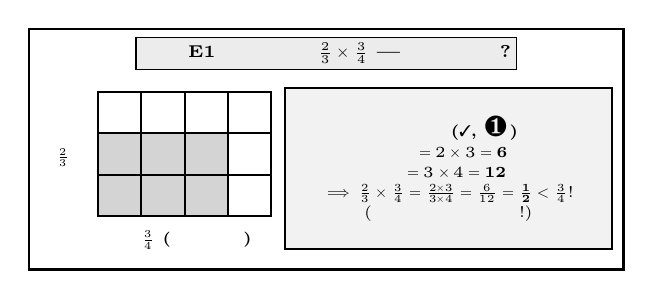
\begin{tikzpicture}[x=0.95cm, y=0.94cm, every node/.style={font=\scriptsize, text=black}]
  \draw[black, line width=0.95pt] (0,0) rectangle (7.95,3.25);
  \node[fill=gray!15, draw=black, line width=0.6pt, inner sep=2pt, font=\fontsize{6.2pt}{7.9pt}\selectfont\bfseries] at (3.975,2.92) {បេសកកម្ម \en{E1}៖ ក្រឡាផ្ទៃសួនបន្លែ $\frac{2}{3}\times\frac{3}{4}$ — តើគុណតែងតែធំជាងមុនឬ?};

  % 4 columns (width 0.58 each = 2.32) x 3 rows (height 0.56 each = 1.68)
  % Shade 3 of 4 cols and 2 of 3 rows -> 6 of 12 cells
  \foreach \c in {0,1,2} {
    \foreach \r in {0,1} {
      \fill[gray!34] (0.92+\c*0.58, 0.72+\r*0.56) rectangle (0.92+\c*0.58+0.58, 0.72+\r*0.56+0.56);
    }
  }
  \foreach \c in {0,...,3} {
    \foreach \r in {0,...,2} {
      \draw[black, line width=0.7pt] (0.92+\c*0.58, 0.72+\r*0.56) rectangle (0.92+\c*0.58+0.58, 0.72+\r*0.56+0.56);
    }
  }
  \node[font=\fontsize{5.5pt}{7.0pt}\selectfont\bfseries] at (2.08,0.40) {ទទឹង $\frac{3}{4}$ (៣ ក្នុង ៤ ជួរឈរ)};
  \node[align=center, font=\fontsize{5.4pt}{6.9pt}\selectfont\bfseries] at (0.46,1.56) {បណ្ដោយ\\$\frac{2}{3}$};

  % Right explanation box
  \draw[black, line width=0.8pt, fill=gray!10] (3.42,0.28) rectangle (7.79,2.45);
  \node[align=center, font=\fontsize{5.6pt}{7.3pt}\selectfont] at (5.605,1.36) {\textbf{រាប់ក្រឡាប្រសព្វ (\ding{51}, \cnum{1})៖}\\ក្រឡាផាត់ពណ៌ $= 2\times 3 = \mathbf{6}$ ក្រឡា\\ក្រឡាសរុប $= 3\times 4 = \mathbf{12}$ ក្រឡា\\$\implies \frac{2}{3}\times\frac{3}{4} = \frac{2\times 3}{3\times 4} = \frac{6}{12} = \mathbf{\frac{1}{2}} < \frac{3}{4}$!\\(\textbf{មិនបាច់}តម្រូវភាគបែងរួមដូចវិធីបូកទេ!)};
\end{tikzpicture}}

% ២. E2 POE 2: សម្រួលខ្វែងមុនគុណ & វែនតាឆ្លុះកត្តារួម (លក្ខណៈបំបែក ទំ.៩)
\newcommand{\figDistributiveRATMUL}{%
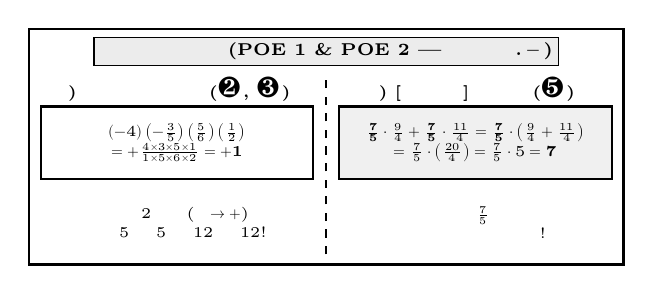
\begin{tikzpicture}[x=0.95cm, y=0.92cm, every node/.style={font=\scriptsize, text=black}]
  \draw[black, line width=0.95pt] (0,0) rectangle (7.95,3.25);
  \node[fill=gray!15, draw=black, line width=0.6pt, inner sep=2pt, font=\fontsize{6.2pt}{7.9pt}\selectfont\bfseries] at (3.975,2.94) {យុទ្ធសាស្ត្រគណនារហ័សដោយដៃ (\en{POE 1 \& POE 2} — សៀវភៅពុម្ព ទំ.៨–៩)};

  \draw[black, dashed, line width=0.65pt] (3.975,0.14) -- (3.975,2.62);

  % Left: Cross-cancel & sign parity (គំរូ ឃ ទំ.៨)
  \node[font=\fontsize{5.7pt}{7.3pt}\selectfont\bfseries] at (1.98,2.42) {១) រាប់សញ្ញាដក និងសម្រួលខ្វែង (\cnum{2}, \cnum{3})};
  \draw[black, line width=0.8pt] (0.16,1.18) rectangle (3.80,2.18);
  \node[align=center, font=\fontsize{5.5pt}{7.1pt}\selectfont] at (1.98,1.68) {$(-4)\left(-\frac{3}{5}\right)\left(\frac{5}{6}\right)\left(\frac{1}{2}\right)$\\$= +\frac{4\times 3\times 5\times 1}{1\times 5\times 6\times 2} = \mathbf{+1}$};
  \node[align=center, font=\fontsize{5.4pt}{6.9pt}\selectfont] at (1.98,0.58) {សញ្ញាដក $2$ កត្តា (គូ $\to +$)\\សម្រួល $5$ នឹង $5$ និង $12$ នឹង $12$!};

  % Right: Common-factor spotlight (គំរូ ក ទំ.៩)
  \node[font=\fontsize{5.7pt}{7.3pt}\selectfont\bfseries] at (5.96,2.42) {២) \textbf{[គូសវង់កត្តារួម]} លក្ខណៈបំបែក (\cnum{5})};
  \draw[black, line width=0.8pt, fill=gray!12] (4.14,1.18) rectangle (7.79,2.18);
  \node[align=center, font=\fontsize{5.5pt}{7.1pt}\selectfont] at (5.965,1.68) {$\mathbf{\frac{7}{5}}\cdot\frac{9}{4} + \mathbf{\frac{7}{5}}\cdot\frac{11}{4} = \mathbf{\frac{7}{5}}\cdot\left(\frac{9}{4}+\frac{11}{4}\right)$\\$= \frac{7}{5}\cdot\left(\frac{20}{4}\right) = \frac{7}{5}\cdot 5 = \mathbf{7}$};
  \node[align=center, font=\fontsize{5.4pt}{6.9pt}\selectfont] at (5.965,0.58) {ទាញកត្តារួម $\frac{7}{5}$ ចេញក្រៅ\\គិតឃើញចម្លើយភ្លាមក្នុង ៥ វិនាទី!};
\end{tikzpicture}}

% ៣. E3/E4 Contrast Box: ចំនួនផ្ទុយ (-a/b) vs. ចំនួនច្រាស (b/a)
\newcommand{\figInverseContrastRATMUL}{%
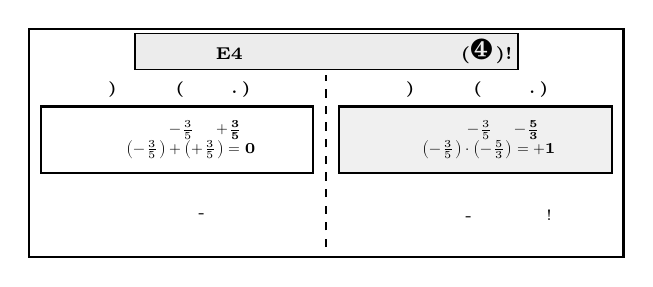
\begin{tikzpicture}[x=0.95cm, y=0.92cm, every node/.style={font=\scriptsize, text=black}]
  \draw[black, line width=0.95pt] (0,0) rectangle (7.95,3.15);
  \node[fill=gray!15, draw=black, line width=0.6pt, inner sep=2pt, font=\fontsize{6.2pt}{7.9pt}\selectfont\bfseries] at (3.975,2.84) {កាតញែកបញ្ញត្តិ \en{E4}៖ កុំច្រឡំ \textbf{ចំនួនផ្ទុយ} ជាមួយនឹង \textbf{ចំនួនច្រាស} (\cnum{4})!};

  \draw[black, dashed, line width=0.65pt] (3.975,0.14) -- (3.975,2.52);

  \node[font=\fontsize{5.7pt}{7.3pt}\selectfont\bfseries] at (1.98,2.32) {១) ចំនួនផ្ទុយ (វិធីបូក ទំ.៦)};
  \draw[black, line width=0.75pt] (0.16,1.16) rectangle (3.80,2.08);
  \node[align=center, font=\fontsize{5.5pt}{7.1pt}\selectfont] at (1.98,1.62) {ចំនួនផ្ទុយនៃ $-\frac{3}{5}$ គឺ $\mathbf{+\frac{3}{5}}$\\ព្រោះ $\left(-\frac{3}{5}\right) + \left(+\frac{3}{5}\right) = \mathbf{0}$};
  \node[align=center, font=\fontsize{5.4pt}{6.9pt}\selectfont] at (1.98,0.58) {ប្ដូរ\textbf{សញ្ញា} រក្សាភាគយក-ភាគបែងដដែល};

  \node[font=\fontsize{5.7pt}{7.3pt}\selectfont\bfseries] at (5.96,2.32) {២) ចំនួនច្រាស (វិធីគុណ ទំ.៩)};
  \draw[black, line width=0.8pt, fill=gray!12] (4.14,1.16) rectangle (7.79,2.08);
  \node[align=center, font=\fontsize{5.5pt}{7.1pt}\selectfont] at (5.965,1.62) {ចំនួនច្រាសនៃ $-\frac{3}{5}$ គឺ $\mathbf{-\frac{5}{3}}$\\ព្រោះ $\left(-\frac{3}{5}\right) \cdot \left(-\frac{5}{3}\right) = \mathbf{+1}$};
  \node[align=center, font=\fontsize{5.4pt}{6.9pt}\selectfont] at (5.965,0.58) {ប្ដូរ\textbf{ទីតាំង}ភាគយក-ភាគបែង រក្សាសញ្ញា!};
\end{tikzpicture}}

% ៤. E5 Diagnostic Cards A-D
\newcommand{\figExitCardsRATMUL}{%
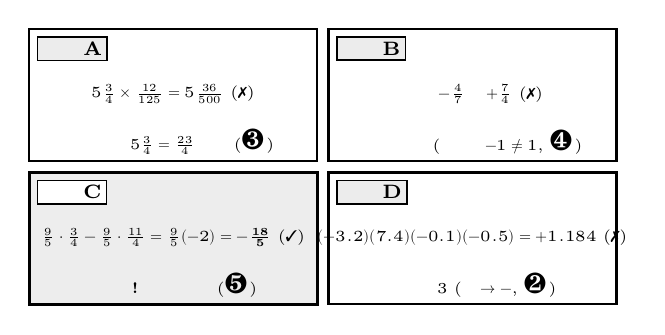
\begin{tikzpicture}[x=0.95cm, y=0.92cm, every node/.style={font=\scriptsize, text=black}]
  \draw[black, line width=0.9pt] (0,1.98) rectangle (3.85,3.80);
  \node[anchor=north west, fill=gray!15, draw=black, line width=0.6pt, inner sep=1.8pt] at (0.10,3.70) {\textbf{ជម្រើស \en{A}}};
  \node[font=\fontsize{5.6pt}{7.3pt}\selectfont] at (1.925,2.90) {$5\frac{3}{4}\times\frac{12}{125} = 5\frac{36}{500}$ (\ding{55})};
  \node[font=\fontsize{5.5pt}{7.1pt}\selectfont] at (1.925,2.24) {ភ្លេចបំប្លែង $5\frac{3}{4}=\frac{23}{4}$ មុនគុណ (\cnum{3})};

  \draw[black, line width=0.9pt] (4.00,1.98) rectangle (7.85,3.80);
  \node[anchor=north west, fill=gray!15, draw=black, line width=0.6pt, inner sep=1.8pt] at (4.10,3.70) {\textbf{ជម្រើស \en{B}}};
  \node[font=\fontsize{5.6pt}{7.3pt}\selectfont] at (5.925,2.90) {ច្រាសនៃ $-\frac{4}{7}$ គឺ $+\frac{7}{4}$ (\ding{55})};
  \node[font=\fontsize{5.5pt}{7.1pt}\selectfont] at (5.925,2.24) {ច្រឡំប្ដូរសញ្ញា (ផលគុណស្មើ $-1 \neq 1$, \cnum{4})};

  \draw[black, line width=1.1pt, fill=gray!14] (0,0) rectangle (3.85,1.82);
  \node[anchor=north west, fill=white, draw=black, line width=0.6pt, inner sep=1.8pt] at (0.10,1.72) {\textbf{ជម្រើស \en{C}}};
  \node[font=\fontsize{5.6pt}{7.3pt}\selectfont] at (1.925,0.92) {$\frac{9}{5}\cdot\frac{3}{4}-\frac{9}{5}\cdot\frac{11}{4}=\frac{9}{5}(-2)=\mathbf{-\frac{18}{5}}$ (\ding{51})};
  \node[font=\fontsize{5.5pt}{7.1pt}\selectfont] at (1.925,0.26) {\textbf{ត្រឹមត្រូវ!} ប្រើលក្ខណៈបំបែក (\cnum{5})};

  \draw[black, line width=0.9pt] (4.00,0) rectangle (7.85,1.82);
  \node[anchor=north west, fill=gray!15, draw=black, line width=0.6pt, inner sep=1.8pt] at (4.10,1.72) {\textbf{ជម្រើស \en{D}}};
  \node[font=\fontsize{5.6pt}{7.3pt}\selectfont] at (5.925,0.92) {$(-3.2)(7.4)(-0.1)(-0.5)=+1.184$ (\ding{55})};
  \node[font=\fontsize{5.5pt}{7.1pt}\selectfont] at (5.925,0.26) {កត្តាដកមាន $3$ (សេស $\to -$, \cnum{2})};
\end{tikzpicture}}

\begin{document}
\fontsize{10pt}{15.2pt}\selectfont

% -------------------- ក្បាលកិច្ចតែងការ --------------------
\begin{center}
  {\muol\fontsize{11pt}{16pt}\selectfont ព្រះរាជាណាចក្រកម្ពុជា}\\[2pt]
  {\muol\fontsize{10pt}{15pt}\selectfont ជាតិ សាសនា ព្រះមហាក្សត្រ}\\[1pt]
  \khmflourish
\end{center}

\vspace{-24pt}
{\muol\fontsize{9.5pt}{12.5pt}\selectfont
មន្ទីរអប់រំ យុវជន និងកីឡា ខេត្តកំពង់ធំ\\
ការិយាល័យអប់រំ យុវជន និងកីឡា ស្រុកកំពង់ស្វាយ\\
អនុវិទ្យាល័យព្រះក្រសាំង}

\vspace{1pt}
\begin{center}
  {\muol\fontsize{10pt}{14pt}\selectfont កិច្ចតែងការបង្រៀន}
\end{center}
\vspace{0pt}

% -------------------- ព័ត៌មានទូទៅ --------------------
{\renewcommand{\arraystretch}{0.98}
\hspace*{3.1cm}%
\begin{tabular}{@{}l l L{11.0cm}@{}}
  - \hspace{0.35cm} មុខវិជ្ជា & : & គណិតវិទ្យា ថ្នាក់ទី៨ (ពីជគណិត) \\
  - \hspace{0.35cm} ចំណងជើងមេរៀន & : & មេរៀនទី១៖ ចំនួនសនិទាន \\
  - \hspace{0.35cm} ចំណងជើងរង & : & ៤. ប្រមាណវិធីគុណនៃចំនួនសនិទាន និងលក្ខណៈ (ទំ.៨–៩) \\
  - \hspace{0.35cm} រយៈពេល & : & ១ ម៉ោងសិក្សា (៥០ នាទី) \\
  - \hspace{0.35cm} បង្រៀនដោយ & : & ហុក ប៊ុនថែន \\
  - \hspace{0.35cm} កាលបរិច្ឆេទ & : & ថ្ងៃសុក្រ ទី២០ ខែវិច្ឆិកា ឆ្នាំ២០២៦ \\
\end{tabular}

\vspace{2pt}

% -------------------- I. វត្ថុបំណង --------------------
\textbf{I.} {\muol វត្ថុបំណង}\\[1pt]
\hspace*{0.55cm}%
\begin{tabular}{@{}l l L{14.2cm}@{}}
  \wcirc \hspace{0.25cm} វិជ្ជាសម្បទា & : & សិស្សប្រាប់រូបមន្តគុណចំនួនសនិទាន ($\frac{a}{b}\cdot\frac{c}{d}=\frac{ac}{bd}$) ក្បួនសញ្ញានៃផលគុណ និយមន័យចំនួនច្រាស ($\frac{a}{b}\cdot\frac{b}{a}=1$) និងលក្ខណៈទាំង ៦ នៃវិធីគុណបានត្រឹមត្រូវតាមសៀវភៅគោល (ទំ.៨–៩) ។ \\
  \wcirc \hspace{0.25cm} បំណិនសម្បទា & : & សិស្សគណនាផលគុណប្រភាគមានសញ្ញា ចំនួនចម្រុះ ចំនួនទសភាគ ដោយសម្រួលខ្វែងមុនគុណ និងប្រើលក្ខណៈផ្គុំ-បំបែកលើសន្លឹកកិច្ចការបានត្រឹមត្រូវ ។ \\
  \wcirc \hspace{0.25cm} ចរិយាសម្បទា & : & សិស្សមានភាពវៃឆ្លាតក្នុងការសង្កេតរកកត្តារួម និងសម្រួលមុនគុណ ជួយសន្សំពេលវេលា និងកាត់បន្ថយកំហុសគណនាលេខធំៗដោយដៃ ។ \\
\end{tabular}

\vspace{2pt}

% -------------------- II. សម្ភារៈឧបទេស --------------------
\textbf{II.} {\muol សម្ភារៈឧបទេស}\\[1pt]
\hspace*{0.55cm}$\bullet$ \hspace{0.35cm} សៀវភៅសិក្សាគោលគណិតវិទ្យាថ្នាក់ទី៨ (ទំ.៨–៩ និងទំ.១២) ក្ដារខៀន ដីស និងសន្លឹកកិច្ចការសិស្ស ស-ខ្មៅ (\en{Worksheet\_RAT\_MUL} ទំព័រ ១–២ គ្មានស្លាយ \en{LCD} គ្មានម៉ាស៊ីនគិតលេខ)

\vspace{2pt}

% -------------------- III. វិធីសាស្រ្តបង្រៀន --------------------
\textbf{III.} {\muol វិធីសាស្រ្តបង្រៀន}\\[1pt]
\hspace*{0.45cm}%
\begin{tabular}{@{}l l L{14.85cm}@{}}
  $\bullet$ \hspace{0.25cm} គោលវិធី & : & សិស្សមជ្ឈមណ្ឌល (បង្រៀនតាមសន្លឹកកិច្ចការស៊ើបអង្កេតជាដៃគូ និងក្ដារខៀន គ្មាន \en{LCD}) \\
  $\bullet$ \hspace{0.25cm} យុទ្ធវិធីបង្រៀន & : & គំរូ \en{5Es} រួមបញ្ចូលក្រឡាផ្ទៃប្រភាគ សម្រួលខ្វែងមុនគុណ \en{(POE 1)} និងវែនតាឆ្លុះកត្តារួម \en{(POE 2)} \\
\end{tabular}
}

\vspace{2pt}

% -------------------- IV. ដំណើរការបង្រៀន --------------------
\textbf{IV.} {\muol ដំណើរការបង្រៀន}

\vspace{1pt}

\renewcommand{\arraystretch}{1.15}
\begin{longtable}{|L{5.50cm}|L{7.90cm}|L{4.80cm}|}
\hline
\rowcolor{headgray}
\multicolumn{1}{|c|}{\muol សកម្មភាពគ្រូ} &
\multicolumn{1}{c|}{\muol ខ្លឹមសារមេរៀន} &
\multicolumn{1}{c|}{\muol សកម្មភាពសិស្ស} \\
\hline
\endfirsthead

\hline
\rowcolor{headgray}
\multicolumn{1}{|c|}{\muol សកម្មភាពគ្រូ} &
\multicolumn{1}{c|}{\muol ខ្លឹមសារមេរៀន} &
\multicolumn{1}{c|}{\muol សកម្មភាពសិស្ស} \\
\hline
\endhead

\hline
\endfoot

\hline
\endlastfoot

% ==================== ជំហានទី១ (2min) ====================
\stepheader{ជំហានទី១ \enbf{(}រដ្ឋបាលថ្នាក់\enbf{)}}
$\bullet$ ពិនិត្យអវត្តមាន អនាម័យ និងសណ្ដាប់ធ្នាប់ថ្នាក់រៀន \timenote{(2 min)}\par\vspace{2pt}
$\bullet$ ចែក \textbf{សន្លឹកកិច្ចការសិស្ស (\en{Worksheet\_RAT\_MUL})} ម្នាក់ ១ សន្លឹក (ផ្កាប់ទុកសិន)
&
$\bullet$ រដ្ឋបាលថ្នាក់ និងការរៀបចំដៃគូសិក្សា (២ នាក់ក្នុង ១ តុ)\par\vspace{2pt}
$\bullet$ សន្លឹកកិច្ចការសិស្ស ស-ខ្មៅ ២ ទំព័រ សម្រាប់បំពេញតាមជំហានមេរៀន
&
$\circ$ ប្រធានថ្នាក់រាយការណ៍អវត្តមាន\par\vspace{2pt}
$\circ$ ទទួលសន្លឹកកិច្ចការ ដាក់ផ្កាប់លើតុ \\[3pt]
\hline

% ==================== ជំហានទី២ (9min: <=3 + 3 + E1 3) ====================
\stepheader{ជំហានទី២ \enbf{(}កិច្ចការផ្ទះ \enbf{+} ទំនាក់ទំនងមេរៀនថ្មី\enbf{)}}
\timenote{កំណែកិច្ចការផ្ទះ ($\le 3\unit{min}$)}\par\vspace{2pt}
$\bullet$ ហៅសិស្ស ២ នាក់ឡើងកែកិច្ចការផ្ទះចំណុច ៣.៣ លើក្ដារខៀន
&
\textbf{១. កំណែកិច្ចការផ្ទះ (ប្រមាណវិធីដកនៃចំនួនសនិទាន)៖}\par\vspace{2pt}
$\bullet$ \textbf{១ក)} $\dfrac{7}{12}-\dfrac{5}{8} = \dfrac{-1}{24}$ \;;\; \textbf{១ខ)} $-\dfrac{3}{14}-\left(-\dfrac{5}{21}\right) = \dfrac{1}{42}$ \;;\; \textbf{១គ)} $\dfrac{-64}{45}$\par\vspace{2pt}
$\bullet$ \textbf{២)} ប្រភាគប្រាក់នៅសល់ $= 1 - \left(\dfrac{1}{2}+\dfrac{1}{10}\right) = 1 - \dfrac{3}{5} = \dfrac{2}{5}$
&
$\circ$ តំណាងសិស្សឡើងកែលើក្ដារខៀន\par\vspace{2pt}
$\circ$ ផ្ទៀងផ្ទាត់ និងកែតម្រូវចូលសៀវភៅ \\[3pt]

\timenote{រំលឹកមេរៀនទាក់ទង (3 min)}\par\vspace{2pt}
$\bullet$ សួររំលឹកក្បួនសញ្ញាគុណចំនួនគត់រ៉ឺឡាទីប៖ «តើ $(-2)\times(-7)$ និង $(-4)\times 3$ ស្មើប៉ុន្មាន?»
&
\textbf{២. រំលឹកគុណចំនួនគត់ និងបំប្លែងទសភាគជាប្រភាគ៖}\par\vspace{2pt}
$\bullet$ ក្បួនសញ្ញាគុណ៖ $(-2)\times(-7) = +14$ \;;\; $(-4)\times 3 = -12$
&
$\circ$ ឆ្លើយផ្ទាល់មាត់៖ $+14$ និង $-12$ \\[3pt]

$\bullet$ សួរបន្តពីប្រភាគស្មើនឹងទសភាគពិសេស៖ «តើ $0.25$, $0.75$ និង $3.8$ សរសេរជាប្រភាគដូចម្ដេច?»
&
$\bullet$ បំប្លែងរហ័ស៖ $0.25 = \dfrac{1}{4}$ \;;\; $0.75 = \dfrac{3}{4}$ \;;\; $3.8 = \dfrac{38}{10} = \dfrac{19}{5}$
&
$\circ$ ឆ្លើយផ្ទាល់មាត់៖ $\frac{1}{4}$, $\frac{3}{4}$ និង $\frac{19}{5}$ \\[3pt]

\fiveE{E1 - Engage} \timenote{(3 min)}\par\vspace{2pt}
$\bullet$ ឱ្យសិស្សផ្ងារសន្លឹកកិច្ចការទំព័រទី១ អានបេសកកម្ម \en{E1}៖ «សួនបន្លែការ៉េ $1\unit{m}^2$ គេយកបណ្ដោយ $\frac{2}{3}\unit{m}$ និងទទឹង $\frac{3}{4}\unit{m}$ ។ តើផ្ទៃដាំស្ពៃ $\frac{2}{3}\times\frac{3}{4}$ ធំជាង ឬតូចជាង $\frac{3}{4}\unit{m}^2$? តើត្រូវតម្រូវភាគបែងរួមដូចវិធីបូកឬទេ?»
&
\textbf{៣. បេសកកម្ម \en{E1} — ក្រឡាផ្ទៃសួនបន្លែ៖}\par\vspace{2pt}
$\bullet$ ពេលគុណប្រភាគសុទ្ធ ($\frac{2}{3}\times\frac{3}{4}=\frac{1}{2}$) ផលគុណអាចតូចជាងតួដើម!\par\vspace{2pt}
$\bullet$ ភ្ជាប់ចូលមេរៀនថ្មី៖ \textbf{៤. ប្រមាណវិធីគុណ និងលក្ខណៈនៃវិធីគុណ (ទំ.៨–៩)}
&
$\circ$ គូសធីកការទស្សន៍ទាយ រាប់ក្រឡាប្រសព្វ $6$ ក្នុង $12$ ក្រឡា ឃើញស្មើ $\frac{1}{2}$! \\[3pt]

& \cfig{\figEngageRATMUL} & \\[3pt]
\hline

% ==================== ជំហានទី៣ (17min: E2 11 + E3 6) ====================
\stepheader{ជំហានទី៣ \enbf{(}ខ្លឹមសារមេរៀនថ្មី\enbf{)}}
\fiveE{E2 - Explore} \timenote{(11 min)}\par\vspace{2pt}
$\bullet$ សរសេរចំណងជើងមេរៀនលើក្ដារខៀន និងណែនាំ \textbf{សកម្មភាពទី១ (\en{POE 1})} លើសន្លឹកកិច្ចការ (ឧទាហរណ៍ទី១, ទី២ និងគំរូ ឃ ទំ.៨)
&
\textbf{៤. ប្រមាណវិធីគុណនៃចំនួនសនិទាន (ទំ.៨–៩) — \en{POE 1}៖}\par\vspace{2pt}
$\bullet$ \textbf{ឧទាហរណ៍ទី១–២ (ទំ.៨)៖} $\dfrac{3}{8}\times 3.8 = \dfrac{3}{8}\times\dfrac{38}{10} = \dfrac{57}{40}$ \;;\; $\left(-\dfrac{2}{3}\right)\left(-\dfrac{7}{15}\right) = \dfrac{14}{45}$
&
$\circ$ កត់ចំណងជើងមេរៀន និងគណនាឧទាហរណ៍ទី១–២ ជាដៃគូ \\[3pt]

$\bullet$ ឱ្យដៃគូរាប់សញ្ញាដក និងសាកល្បងសម្រួលខ្វែងមុនគុណលើ \textbf{លំហាត់គំរូ ឃ} (ទំ.៨)
&
$\bullet$ \textbf{គំរូ ឃ (ទំ.៨)៖} $(-4)\left(-\dfrac{3}{5}\right)\left(\dfrac{5}{6}\right)\left(\dfrac{1}{2}\right) = \left[(-4)\left(\dfrac{1}{2}\right)\right]\left[\left(-\dfrac{3}{5}\right)\left(\dfrac{5}{6}\right)\right] = (-2)\left(-\dfrac{1}{2}\right) = \graybox{$1$}
$
&
$\circ$ រកឃើញថាការសម្រួលខ្វែងមុនគុណ លឿនជាងការគុណលេខធំឆ្ងាយណាស់! \\[3pt]

$\bullet$ ណែនាំ \textbf{សកម្មភាពទី២ (\en{POE 2} — វែនតាឆ្លុះកត្តារួម)} តាម \textbf{លំហាត់គំរូ ក} (ទំ.៩)៖\par\vspace{2pt}
\hspace*{0.3em}-- \textbf{ទស្សន៍ទាយ (\en{P})៖} «តើចាំបាច់គុណដាច់ៗពីគ្នា ចំពោះ $\frac{7}{5}\cdot\frac{9}{4}+\frac{7}{5}\cdot\frac{11}{4}$ ឬអាចទាញកត្តារួម $\frac{7}{5}$?»
&
\textbf{លក្ខណៈនៃវិធីគុណ (ទំ.៩) — \en{POE 2}៖}\par\vspace{2pt}
$\bullet$ \textbf{គំរូ ក (ទំ.៩)៖} $\dfrac{7}{5}\cdot\dfrac{9}{4}+\dfrac{7}{5}\cdot\dfrac{11}{4} = \dfrac{7}{5}\cdot\left(\dfrac{9}{4}+\dfrac{11}{4}\right) = \dfrac{7}{5}\cdot\left(\dfrac{20}{4}\right) = \dfrac{7}{5}\cdot 5 = \graybox{$7$}$
&
$\circ$ គូសវង់កត្តារួម $\frac{7}{5}$ លើសន្លឹកកិច្ចការ និងឃើញចម្លើយស្មើ $7$ ភ្លាម! \\[3pt]

& \cfig{\figDistributiveRATMUL} & \\[3pt]

\fiveE{E3 - Explain} \timenote{(6 min)}\par\vspace{2pt}
$\bullet$ ហៅតំណាងដៃគូឡើងបង្គុំរូបមន្តទូទៅនៃប្រមាណវិធីគុណ (ទំ.៨) និងសម្គាល់ក្បួនសញ្ញា (ទំ.៩)
&
\textbf{សំយោគបញ្ញត្តិ និងធនាគារហេតុផល \en{B\&W} (\cnum{1}--\cnum{5})៖}\par\vspace{2pt}
$\bullet$ \textbf{ជាទូទៅ (ទំ.៨)៖} $\dfrac{a}{b}\cdot\dfrac{c}{d} = \dfrac{ac}{bd}$ ($b,d\neq 0$) \;;\; \textbf{សញ្ញា៖} ដូចគ្នា $\to +$, ផ្ទុយគ្នា $\to -$
&
$\circ$ កត់ត្រារូបមន្តប្រអប់ «ជាទូទៅ» និងក្បួនសញ្ញាលើសន្លឹកកិច្ចការ \\[3pt]

$\bullet$ សង្ខេបលក្ខណៈទី១ ដល់ទី៤ នៃវិធីគុណចំនួនសនិទាន (សៀវភៅពុម្ព ទំ.៩)
&
$\bullet$ \textbf{លក្ខណៈទី១–ទី៤ (ទំ.៩)៖} (១) ផលគុណជាចំនួនសនិទាន; (២) \textbf{ត្រឡប់} ($\frac{a}{b}\cdot\frac{c}{d}=\frac{c}{d}\cdot\frac{a}{b}$);\par\vspace{1.5pt}
(៣) \textbf{ផ្គុំ}; និង (៤) \textbf{ធាតុណឺតគឺ $1$} ($\frac{a}{b}\cdot 1 = \frac{a}{b}$) ។
&
$\circ$ ប្រៀបធៀបលក្ខណៈវិធីគុណនឹងវិធីបូក \\[3pt]

$\bullet$ សង្កត់ធ្ងន់លើលក្ខណៈទី៥ (\textbf{ចំនួនច្រាស}) និងទី៦ (\textbf{លក្ខណៈបំបែក})
&
$\bullet$ \textbf{លក្ខណៈទី៥–ទី៦ (ទំ.៩)៖} (៥) \textbf{ចំនួនច្រាស} $\dfrac{a}{b}\cdot\dfrac{b}{a}=1$ ($a,b\neq 0$);\par\vspace{1.5pt}
(៦) \textbf{បំបែក} $\dfrac{a}{b}\left(\dfrac{c}{d}\pm\dfrac{e}{f}\right)=\dfrac{a}{b}\cdot\dfrac{c}{d}\pm\dfrac{a}{b}\cdot\dfrac{e}{f}$
&
$\circ$ បំពេញប្រអប់ចំនួនច្រាស និងលក្ខណៈបំបែកលើសន្លឹកកិច្ចការ \\[3pt]

$\bullet$ កត់ធនាគារហេតុផល \cnum{1}--\cnum{3} លើក្ដារខៀន សម្រាប់ការគុណរហ័សដោយដៃ
&
\cnum{1} យកភាគយកគុណភាគយក និងភាគបែងគុណភាគបែង ($\frac{a}{b}\cdot\frac{c}{d}=\frac{ac}{bd}$) ។\par\vspace{1.5pt}
\cnum{2} រាប់ចំនួនកត្តាអវិជ្ជមានជាមុន៖ ចំនួនគូ $\to +$ ; ចំនួនសេស $\to -$ ។\par\vspace{1.5pt}
\cnum{3} បំប្លែងចំនួនចម្រុះ/ទសភាគជាប្រភាគសិន រួចសម្រួលខ្វែងមុនគុណ ។
&
$\circ$ ផ្ទៀងផ្ទាត់ហេតុផល \cnum{1}--\cnum{3} លើសន្លឹកកិច្ចការ \\[3pt]

$\bullet$ បញ្ជាក់ហេតុផល \cnum{4}--\cnum{5} សម្រាប់ចំនួនច្រាស និងលក្ខណៈបំបែក-ផ្គុំ
&
\cnum{4} ចំនួនច្រាសនៃ $\frac{a}{b}$ គឺ $\frac{b}{a}$ ដែល $\frac{a}{b}\cdot\frac{b}{a}=1$ (រក្សាសញ្ញាដដែល; $0$ គ្មានច្រាសទេ) ។\par\vspace{1.5pt}
\cnum{5} លក្ខណៈបំបែក/ផ្គុំ៖ គូសវង់ទាញកត្តារួម $\frac{a}{b}$ ចេញក្រៅ ឬផ្គុំគូសម្រួលដាច់ ។
&
$\circ$ ធ្វើលំហាត់ត្រួតពិនិត្យរហ័សនៅបាតទំព័រទី១ \\[3pt]
\hline

% ==================== ជំហានទី៤ (20min: E4 10 + E5 10) ====================
\stepheader{ជំហានទី៤ \enbf{(}ពង្រឹង និងពង្រីកចំណេះដឹង\enbf{)}}
\fiveE{E4 - Elaborate} \timenote{(10 min)}\par\vspace{2pt}
$\bullet$ ឱ្យសិស្សបើកសន្លឹកកិច្ចការទំព័រទី២ (ផ្នែកទី៣) ស៊ើបអង្កេត \textbf{លំហាត់គំរូ ក, គ} (ទំ.៨)
&
\textbf{១. លំហាត់គំរូ (ទំ.៨ និងទំ.៩)៖}\par\vspace{2pt}
$\bullet$ \textbf{ក) ទំ.៨ ក៖} $0.25\times 48 = \dfrac{1}{4}\times 48 = \graybox{$12$}$ \;;\; \textbf{ខ) ទំ.៨ ខ៖} $245.4\times 5.3 = \mathbf{1300.62}$\par\vspace{2pt}
$\bullet$ \textbf{គ) ទំ.៨ គ៖} $(-3.2)(7.4)(-0.1)(-0.5) = [( -3.2 )(-0.5)][(7.4)(-0.1)] = (1.6)(-0.74) = \graybox{$-1.184$}$
&
$\circ$ បំពេញជំហានគណនាដោយប្រើប្រភាគពិសេស និងរាប់កត្តាដក $3$ តួ \\[3pt]

$\bullet$ បន្តដឹកនាំ \textbf{លំហាត់គំរូ ខ, គ} (ទំ.៩ — លក្ខណៈបំបែក និងផ្គុំ) និងសំណួរ \en{EIA Looking-Back}
&
$\bullet$ \textbf{ឃ) ទំ.៩ ខ៖} $\dfrac{4}{5}\cdot\dfrac{9}{4}-\dfrac{7}{8}\cdot\dfrac{4}{5} = \dfrac{4}{5}\left(\dfrac{18-7}{8}\right) = \dfrac{4}{5}\cdot\dfrac{11}{8} = \graybox{$\dfrac{11}{10}$} \quad (\text{\cnum{5}})$\par\vspace{2pt}
$\bullet$ \textbf{ង) ទំ.៩ គ៖} $\dfrac{-3}{5}\left(\dfrac{7}{8}\cdot\dfrac{10}{-3}\right) = \dfrac{7}{8}\left(\dfrac{-3}{5}\cdot\dfrac{10}{-3}\right) = \dfrac{7}{8}\cdot 2 = \graybox{$\dfrac{7}{4}$}$\par\vspace{3pt}
&
$\circ$ ឆ្លើយសំណួរ \en{EIA Looking-Back} ញែកចំនួនផ្ទុយ និងចំនួនច្រាស \\[4pt]

& \cfig{\figInverseContrastRATMUL} & \\[3pt]

\fiveE{E5 - Evaluate} \timenote{(10 min)}\par\vspace{2pt}
$\bullet$ ឱ្យសិស្សធ្វើលំហាត់ \textbf{ប្រតិបត្តិ} (ទំ.៩ ផ្នែកលើ ក, ខ, គ) លើសន្លឹកកិច្ចការ រួចផ្ទៀងផ្ទាត់ជាដៃគូ (\en{Pause-Review})
&
\textbf{២. ប្រតិបត្តិ (ទំ.៩ ផ្នែកលើ និងផ្នែកក្រោម)៖}\par\vspace{2pt}
$\bullet$ \textbf{ទំ.៩ លើ៖} ក) $0.75\times\dfrac{13}{125}=\dfrac{3}{4}\times\dfrac{13}{125}=\mathbf{\dfrac{39}{500}}$ \;;\; ខ) $5\dfrac{3}{4}\times\dfrac{12}{125}=\dfrac{23}{4}\times\dfrac{12}{125}=\mathbf{\dfrac{69}{125}}$\par\vspace{2pt}
$\bullet$ គ) $\left(-\dfrac{1}{3}\right)\left(\dfrac{3}{5}\right)(0.5)(0.2) = \left(-\dfrac{1}{5}\right)(0.1) = \mathbf{-0.02}$ (ឬ $-\dfrac{1}{50}$)
&
$\circ$ គណនាប្រតិបត្តិផ្នែកលើដោយដៃ និងផ្ទៀងផ្ទាត់ការសម្រួលខ្វែង \\[3pt]

$\bullet$ បន្តផ្ទៀងផ្ទាត់ \textbf{ប្រតិបត្តិ ទំ.៩ ផ្នែកក្រោម} (ប្រើលក្ខណៈបំបែក និងផ្គុំ) និងបិទបេសកកម្ម \en{E1}
&
$\bullet$ \textbf{ទំ.៩ ក្រោម៖} ក) $\dfrac{9}{5}\left(\dfrac{3-11}{4}\right)=\mathbf{-\dfrac{18}{5}}$ \;;\; ខ) $\dfrac{2}{3}\left(\dfrac{6-7}{8}\right)=\mathbf{-\dfrac{1}{12}}$ \;;\; គ) $\left(-\dfrac{3}{7}\cdot\dfrac{10}{12}\right)\cdot\dfrac{6}{10}=\mathbf{-\dfrac{3}{14}}$\par\vspace{2pt}
$\bullet$ \textbf{បិទ \en{E1}៖} ផ្ទៃដាំស្ពៃគឺ $\dfrac{2}{3}\times\dfrac{3}{4} = \dfrac{6}{12} = \mathbf{\dfrac{1}{2}\unit{m}^2}$ \mbox{(\cnum{1}, \cnum{3})!}
&
$\circ$ តំណាងដៃគូបកស្រាយលក្ខណៈបំបែក និងបិទបញ្ចប់បេសកកម្ម \en{E1} \\[3pt]

$\bullet$ វាយតម្លៃរហ័ស \textbf{៦០ វិនាទី}៖ ឱ្យសិស្សគូសវង់ជម្រើសត្រឹមត្រូវក្នុងប្រអប់ \en{A--D} និងបំពេញសំបុត្រចេញ
&
\textbf{៣. វិនិច្ឆ័យកំហុសរហ័ស (\en{A--D})៖} ចម្លើយត្រឹមត្រូវគឺ \graybox{\textbf{ជម្រើស \en{C}}} ($-\frac{18}{5}$) ។\par\vspace{2pt}
(\en{A} ភ្លេចបំប្លែងចំនួនចម្រុះ; \en{B} ច្រឡំច្រាសប្ដូរសញ្ញា; \en{D} ច្រឡំសញ្ញាកត្តាដក $3$ តួ)
&
$\circ$ គូសវង់ជម្រើស \en{C} និងបំពេញសំបុត្រចេញមុនបញ្ចប់ម៉ោង \\[3pt]

& \cfig{\figExitCardsRATMUL} & \\[3pt]
\hline

% ==================== ជំហានទី៥ (<=2min) ====================
\stepheader{ជំហានទី៥ \enbf{(}កិច្ចការផ្ទះ \enbf{+} បណ្ដាំផ្ញើ\enbf{)}}
\timenote{ចំណាយពេលឱ្យតិចបំផុតកុំឱ្យលើស 2 min}\par\vspace{2pt}
$\bullet$ ណែនាំកិច្ចការផ្ទះនៅផ្នែកទី៥ នៃសន្លឹកកិច្ចការ (សៀវភៅពុម្ព ទំ.១២ \#10) និងផ្ដាំផ្ញើឱ្យអានមុនចំណុច \textbf{៥. ប្រមាណវិធីចែកនៃចំនួនសនិទាន} (ទំ.១០)
&
\centerline{\muol កិច្ចការផ្ទះ}\par\vspace{2pt}
$\bullet$ \textbf{លំហាត់ ១ (ទំ.១២ \#10ក,ខ)៖} គណនា៖ ក) $-\dfrac{4}{5}\cdot\left(\dfrac{11}{17}\cdot\dfrac{10}{16}\right)$ \quad ខ) $-\left(\dfrac{11}{13}\cdot\dfrac{17}{16}\right)\cdot\dfrac{26}{51}$\par\vspace{2pt}
$\bullet$ \textbf{លំហាត់ ២ (ទំ.១២ \#10ឃ,ច)៖} ក) $-\dfrac{11}{8}\cdot\dfrac{21}{22}+\dfrac{17}{16}\cdot\dfrac{21}{22}$ \quad ខ) $\left(-\dfrac{11}{21}\right)\cdot\dfrac{3}{7}+\left(\dfrac{-3}{7}\right)\cdot\left(-\dfrac{11}{21}\right)$\par\vspace{2pt}
$\bullet$ \textbf{បណ្ដាំផ្ញើ៖} អានមុនចំណុច \textbf{៥. ប្រមាណវិធីចែកនៃចំនួនសនិទាន} (សៀវភៅពុម្ព ទំ.១០) ។
&
$\circ$ កត់ត្រាកិច្ចការផ្ទះ និងទទួលបណ្ដាំផ្ញើដោយសណ្ដាប់ធ្នាប់ \\[3pt]
\end{longtable}

% -------------------- កាលបរិច្ឆេទ និងហត្ថលេខា --------------------
\vspace{2pt}
\hfill
\begin{minipage}{9.8cm}
  {\centering
    ថ្ងៃសុក្រ ១១កើត ខែកត្តិក ឆ្នាំមមី អដ្ឋស័ក ពុទ្ធសករាជ ២៥៧០\\[2pt]
    ត្រូវនឹងថ្ងៃទី២០ ខែវិច្ឆិកា ឆ្នាំ២០២៦\\[3pt]
    {\muol គ្រូបង្រៀន}\par}
  \vspace{28pt}
  \hfill{\muol ហុក ប៊ុនថែន}\hspace*{1.4cm}
\end{minipage}

\end{document}
